\documentclass[12pt, a4paper, lithuanian, final]{article}

\usepackage{hyperref}
\usepackage{graphicx}
\usepackage{float}
\usepackage{placeins}
\usepackage{gensymb}
\usepackage{xcolor}
\usepackage{listings}
\usepackage{amsmath}
\usepackage{textgreek}
\usepackage{mathtools}
\usepackage[obeyFinal]{easy-todo}
\usepackage[utf8]{inputenc}
\def\LTfontencoding{L7x}
\usepackage[\LTfontencoding]{fontenc}
\usepackage[lithuanian]{babel}
%\usepackage{times}

%\renewcommand{\sfdefault}{uhv}
%\renewcommand{\rmdefault}{utm}
%\renewcommand{\ttdefault}{ucr}

\usepackage{VUMIF}

%Kodo highlitinimo configas
\lstset{basicstyle=\ttfamily,
	showstringspaces=false,
	commentstyle=\color{red},
	keywordstyle=\color{blue}
	}


% Titulinio puslapio reikalai
\vumifdept{Programų sistemų katedra}
\vumifpaper{Bakalaurinis darbas}
\title{Autonominis ketursraigčio skrydžio valdymas\\Autonomus Control of Quadcopter Flight}
\author{
    4 kurso 1 grupės studentas \\
    Rytis Karpuška
}

\supervisor{Irus Grinis, lekt.}
\reviewer{Vytautas Valaitis}
\date{Vilnius \\
	2014}


\begin{document}

%titulinis ir turinys
\maketitle
\tableofcontents



\vumifsectionnonum{Įvadas}



\section{Ketursraigčio techninė įranga}
Įprasto ketursraigčio techninė struktūra yra palyginus lengvai suprojektuojama bei pagaminama tačiau to negalima pasakyti apie programinę įrangą, bei algoritmus valdančius skrydį.



\subsection{Rėmas, varikliai ir propeleriai}
Ketursraigtis susideda iš "`X"' formos rėmo, kurio galuose yra po elektrinį bešepetėlinį variklį su propeleriu.
Priešingai nei įprastuose sraigtasparniuose, šių propelerių atakos kampas nėra reguliuojamas, o tai leidžia stipriai supaprastinti skraidyklės techninę struktūrą ir atsisakyti sudėtingų mechaninių dalių.
Varikliai skirstomi į dvi grupes iš kurių viena sukasi pagal laikrodžio rodyklę, kita -- prieš laikrodžio rodyklę.
Šių variklių sukimosi greitis yra reguliuojamas siekiant išgauti tinkamą sukamąją bei keliamąją jėgas.

\begin{figure}[H]
\begin{center}
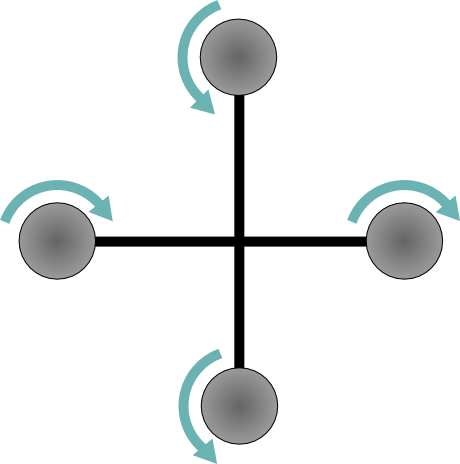
\includegraphics[width=0.5\textwidth]{img/rotor-direction.png}
\caption{Ketursraigčio rėmo ir variklių išdėstymas. Jų sukimosi kryptys.}
\end{center}
\end{figure}

Šio darbo tikslams pasiekti buvo nupirktas "`HobbyKing x525"' 600mm skersmens rėmas, pagamintas iš aliuminio ir stiklo pluošto.
Taip pat elektriniai bešepetėliniai 160W galios varikliai "`Turnigy D2822"' ir 8 colių ilgio, bei 4 laipsnių atakos kampo propeleriai.


\subsection{Valdymo elektronika}
Stabilaus skrydžio išlaikymas ketursraigtyje yra per sudėtinga užduotis žmogui (pilotui) todėl pasitelkiama pagalbinė elektronika palengvinanti ketursraigčio valdymą.

Valdymo elektronikai išskiriami tokie uždaviniai:
\begin{itemize}
	\item Skrydžio stabilizavimas bei kontrolė
	\item Ryšio su pilotu arba valdančia sistema palaikymas
	\item Sugeneruoti galios signalus reikalingus varikliams
\end{itemize}

\paragraph{Skrydžio stabilizavimas bei kontrolė}
Skrydžio stabilizavimui bei kontrolei atlikti naudojami sensoriai pagal kurių duomenis yra paskaičiuojami kokių korekcinių veiksmų reikia imtis norint įgyvendinti piloto ar valdančios sistemos komandas.
Išskiriami svarbiausi parametrai yra tikslumas bei greitis.

Atsižvelgiant į rekalavimus šiems parametrams, buvo parinktas kompanijos "`STMicroelectronics"' procesorius "`STM32F401"' bei kompanijos "`InvenSense"' sensorius "`MPU6050"'

\paragraph{Ryšio su pilotu arba valdančia sistema palaikymas}
Ryšio palaikymas parametrizuojamas pagal duomenų persiuntimo greitį ir latenciją, bei veikimo ribas.
Ketursaigčio atveju persiunčami duomenys yra tik valdymo signalai iš piloto arba valdančios sistemos, todėl buvo pasirinktas GSM ryšys.
Taip pat "`Raspberry pi"' kompiuteris su "`Linux"' operacine sistema atlikdavo viską kas reikalinga GSM ryšiui palaikyti.

\paragraph{Galios signalų generavimas}
Bešepetėliniai varikliai reikalauja trijų galio signalų jų sukimuisi palaikyti.
Šiam tiklui buvo nupirkti 18A elektroniniai greičio valdikliai galintys suvaldyti apie 200W galios, tad puikiai tinkantys 160W galios varikliams.

\begin{figure}[H]
\begin{center}
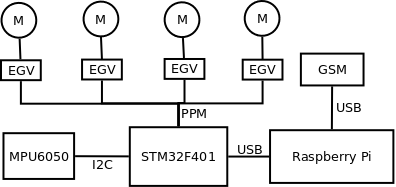
\includegraphics[width=0.5\textwidth]{img/elektronikosSchema.png}
\caption{Ketursraigčio elektronikos sudedamųjų dalių schema.}
\end{center}
\end{figure}




\section{Matematinis skrydžio modelis}



\subsection{Lokali ir globali koordinačių sistemos}
Pravartu apibrėžti lokalią ir globalią koordinačių sistemas, kuriose nagrinėsime ketursraigčio dinamiką.
Lokalioje koordinačių sistemoje x ir y ašis yra sulygiuota su ketursraigčio rėmo strypais, kur $X$ rodo pirmojo variklio kryptimi, $Y$ - antrojo.
Globali sistema yra susieta su žemės gravitaciniu laiku, ir toje sistemoje gravitacinio lauko vektorius nukreiptas priešinga $Z$ ašiai kryptimi.

\begin{figure}[H]
\begin{center}
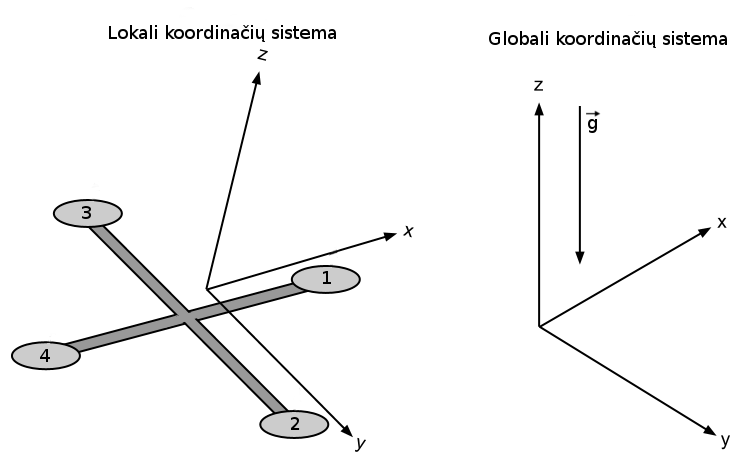
\includegraphics[width=1.0\textwidth]{img/Quadcopter_Coordinates.png}
\caption{Lokalios ir Globalios koordinačių sistemos palyginimas.}
\end{center}
\end{figure}


Konvertavimas tarp šių koordinačių sistemų bus vykdomas kvaternionų pagalba (žr.: TODO\_SKYR\_NR):

\begin{equation}
	q_{l} = q_{p} * q_{g} * q_{p}^{-1}
\end{equation}

ir į priešingą pusę:

\begin{equation}
	q_{g} = q_{p}^{-1} * q_{l} * q_{p}
\end{equation}

Čia $q_{g}$ -- tašką arba vektorių globalioje koordinačių sistemoje atvaizduojantis kvaternionas, $q_{l}$ -- tašką arba vektorių lokalioje koordinačių sistemoje atvaizduojantis kvaternionas, $q_{p}$ -- kampinės pozicijos kvaternionas (žr.: TODO\_SKYR\_NR).





\subsection{Keliamoji jėga}

Ketursaigtis sukuria keliamąją jėgą priversdamas judėti orą žemyn.
Kadangi naudojami nekintamo atakos kampo propeleriai, keliamoji jėga reguliuojama valdant propelerių sukimosi greitį.
pagal (TODO\_REFERENCE) keliamoji jėga gali būti apskaičiuota:
\begin{equation}
	T = C * \omega^2
\end{equation}

Kur $T$ yra keliamoji jėga niutonais vienam varikliui, $C$ yra konstanta priklausanti tik nuo propelerio nekintamų savybių, o $\omega$ yra variklių sukimosi greitis.

Taip pat galime paskaičiuoti bendrąją keliamąją jėga visiems varikliams.

\begin{equation}
	T = \displaystyle\sum_{i=1}^{4} T_i = \left[
		\begin{array}{c}
			C_{1} * \omega_{1}^2 - C_{4} * \omega_{4}^2 \\
			C_{2} * \omega_{2}^2 - C_{3} * \omega_{3}^2\\
			\displaystyle\sum_{i=1}^{4} C_i * \omega_i^2
		\end{array}
	\right]
\end{equation}

Šiuo atveju $T$ yra keliamosios galios vektorius lokalioje koordinačių sistemoje.
Verta pastebėti, kad esant nevienodiems $\omega_{1}, \omega_{4}$ arba $\omega_{2}, \omega_{3}$ sukuriama jėga sukanti ketursraigtį apie jo lokalią $Y$ arba $X$ ašį atitinkamai.

O skaičiuojant globalioje koordinačių sistemoje:

\begin{equation}
q_{tl} = \left[
		\begin{array}{c}
			0\\
			T_x\\
			T_y\\
			T_z\\
		\end{array}
		\right]
\end{equation}
\begin{equation}
	q_{tg} = q_{p}^{-1} * q_{tl} * q_{p}
\end{equation}
\begin{equation}
	T_g = \left[
		\begin{array}{c}
			q_{tg_x} \\
			q_{tg_y} \\
			q_{tg_z}
		\end{array}
	\right]
\end{equation}

Čia $q_{tl}$ yra kvaternionas reprezentuojantis keliamosios jėgos vektorių lokalioje koordinačių sistemoje, $q_{p}$ kvaternionas reprezentuojantis pasukimą nuo globalios iki lokalios koordinačių sistemos (žr.: TODO\_SECT\_NR), $q_{tg}$ -- keliamosios jėgos vektorių atvaizduojantis kvaternionas globalioje koordinačių sistemoje, $T_g$ -- keliamosios jėgos vektorius globalioje koordinačių sistemoje.





\subsection{Sukamoji jėga}

Besisukant propeleriams oro trintis į mentes sukelia papildomą jėgą, kuri veikia ketursraigčio rėmą.
Kiekvienam iš variklių ši jėga yra nukreipta priešinga kryptimi nei sukasi variklis.
Norint išvengti nevaldomo ketursraigčio sukimosi, parenkami du propeleriai skirti suktis pagal laikrodžio rodyklę ir du propeleriai skirti suktis prieš laikrodžio rodyklę, varikliai sujungiami taip, kad jų sukimosi kryptis atitiktų propelerį ir oro srautas būtų nukreiptas žemyn.
Konkrečiu atveju varikliai 1 ir 4 sukasi prieš laikrodžio rodyklę, o varikliai 2 ir 3 -- pagal.
Šitaip vienos krypties jėga kompensuoja kitą ir tampa įmanomas skrydis be sukimosi apie $Z$ ašį lokalioje koordinačių sistemoje.

Šią jėgą modeliuosime tiesiškai priklausančią nuo sukimosi greičio:
\begin{equation}
	F_{tq} = -\omega * C
\end{equation}

Čia $C$ yra konstata priklausanti tik nuo propelerio savybių. Sukamoji jėga yra sukeliama oro pasipriešinimo, todėl ji yra priešinga judėjimo krypčiai $\omega$.


\begin{figure}[H]
\begin{center}
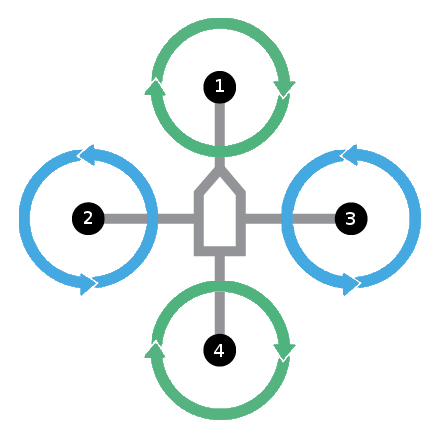
\includegraphics[width=0.75\textwidth]{img/quadcopter-torque.png}
\caption{Jėgos sukeliamos dėl oro trinties į propelerius.}
\end{center}
\end{figure}

Verta pastebėti, kad varikliai skaidomi grupėmis pagal sukimosi kryptį. Tos pačios sukimosi krypties variklis sukuria tos pačios krypties sukamąją jėgą, tik centras kitoje vietoje. Tačiau rėmo atžvilgiu šias grupes galima nagrinėti kaip vieną jėga.
Tokiu atveju turime dvi jėgas priešingų krypčių (žr.: TODO\_PAV\_REFERENCE).

\begin{figure}[H]
\begin{center}
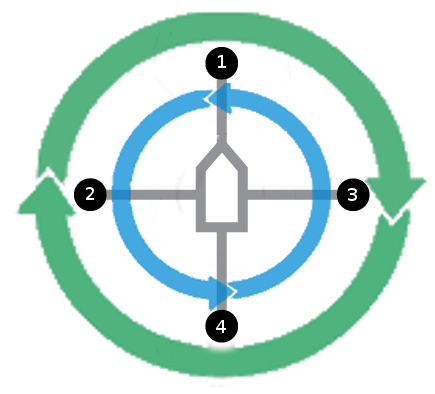
\includegraphics[width=0.75\textwidth]{img/quadcopter-torque-grouped.png}
\caption{Jėgos sukeliamos dėl oro trinties į propelerius.}
\end{center}
\end{figure}

Šiuo atveju vidinės rodyklės rodo 2 ir 3 variklių sukamąsias jėgas, o išorinis -- 1 ir 4 (žr.: TODO\_REFERENCE\_I\_IMAGE).
Verta pastebėti, kad rodyklių storis nėra susijęs su jėgos dydžiu.

Sukamosios jėgos neturi vieningos krypties, kuri nepriklausytų nuo stebėjimo pozicijos, todėl ji bus išreikšta ne vektorine forma, todėl nagrinėsime sukamosios jėgos dydį ties varikliais.
Taip pat, sakysime, kad jėga yra teigiama kai sukamasi apie lokalią $Z$ ašį pagal laikrodžio rodyklę.
Tada gauname, kad sukamoji jėga:
\begin{equation}
	F_{tq_{1,4}} = C * (\omega_{1} + \omega_{4})
\end{equation}
\begin{equation}
	F_{tq_{2,3}} = -C * (\omega_{2} + \omega_{3})
\end{equation}

Ir bendra jėga:
\begin{equation}
	F_{tq} = F_{tq_{1,4}} - F_{tq_{2,3}} = C * (\omega_{1} - \omega_{2} - \omega_{3} + \omega_{4})
\end{equation}

Šias jėgų kryptis atitinkamai galime pasukti pagal $q_{p}$ tik priešinga kryptimi, ir gausime jėgą globalioje koordinačių sistemoje.
Verta pastebėti, kad šių jėgų kryptys visada sutaps su propelerių plokštuma.

\subsection{Bendras judėjimo modelis}

Ketursraigčio skrydžio judėjimai apibrėžti reikia įsivesti gravitacijos kryptį.

\begin{equation}
	g_{g} =  \left[
		\begin{array}{c}
			0 \\
			0 \\
			-9.8
		\end{array}
	\right]
\end{equation}

$g_{g}$ yra apibrėžtas globalioje koordinačių sistemoje.

Tuomet bendra jėga veikianti ketursraigtį:

\begin{equation}
	F_{g} = T_{g} - m*g_{g}
\end{equation}

Čia $m$  yra ketusraigčio bendra masė.

Toliau pagal antrąjį Niutono dėsnį:
\begin{equation}
	a_{g} = \dfrac{F_{g}}{m}
\end{equation}

kur $a$ yra pagreičio vektorius globalioje koordinačių sistemoje.

Toliau randamas greitis bei pozicijos priklausomybė nuo laiko:
\begin{equation}
	v_{g} = a_{g} * \Delta t
\end{equation}
\begin{equation}
	x_{g} = a_{g} * \Delta t ^2
\end{equation}

Tais pačiais principais randama ir kampinė pozicija.




%TODO:%
\textbf{IDEA::: perrašyti modelį įvedant funkcijų priklausomybę nuo laiko t}



\section{Kampinės padėties skaičiavimas}

Ketursraigčio valdymo algoritmai yra tiesiogiai priklausomi nuo kampinės padėties, bet nėra sensorių leidžiančių tai išmatuoti tiesiogiai, todėl šiame skyrelyje apibūdinami principai pagal kuriuos yra apskaičiuojama ketursraigčio kampinė pozicija globalios koordinačių sistemos atžvilgiu.

\subsection{Kvaternionai}

Kvaternionai matematikoje yra skaičių sistema kurį išplėčia įprastus kompleksinius skaičius.
Kvaternionas tai yra keturmatis vektorius

\begin{equation}
	q = \left[
		\begin{array}{c}
			w \\
			i \\
			j \\
			k
		\end{array}
	\right]
\end{equation}

kur $w$ yra sveikoji dalis, o $i$, $j$, $k$, yra menamosios.


Menamosios dalys tarpusavyje susiejamos pagal:
\begin{equation}
	i^2 = j^2 = k^2 = ijk = -1
\end{equation}

o daugindami kiekvieną elementą su kiekvienu gauname tokį sąryšį:

\begin{center}
\begin{tabular}{ | c | c | c | c | c | }
	\hline
	\textbf{x} & \textbf{1} & \textbf{i} & \textbf{j} & \textbf{k} \\
	\hline
	\textbf{1} & 1 & i & j & k \\
	\hline
	\textbf{i} & i & -1 & k & -j \\
	\hline
	\textbf{j} & j & -k & -1 & i \\
	\hline
	\textbf{k} & k & j & -i & -1 \\
	\hline
\end{tabular}
\end{center}


\textbf{TODO: daugiau papasakoti apie kvaternionus ir jų išreiškimo būdą}
Toliau kvaternionai bus apibrėžti taip:

\begin{equation}
	q = \left[
		\begin{array}{c}
			w \\
			x * i \\
			y * j \\
			z * k
		\end{array}
	\right]
\end{equation}

kur $w$ yra sveikoji dalis, $x$, $y$, $z$ yra sveikieji daugikliai, o $i$, $j$, $k$ yra menamosios kvaterniono dalys.


\paragraph{Daugyba}

Kvaternionų daugyba matematiškai išreiškiama kaip jo elementų sudauginimas prastinant pagal distributyvumo taisyklę, ir tai vadinama Hamiltono produktu.

\begin{equation}
	q_1 * q_2 = \left[ w_1, x_1 i_1, y_1j_1, z_1k_1 \right] * \left[ w_1, x_1 i_1, y_1j_1, z_1k_1 \right]
\end{equation}

Verta pastebėti, kad čia nėra paprasta vektorinė daugyba.
Daugyba apibrėžiama taip:

\begin{equation}
	q_1 * q_2 = \left[
		\begin{array}{c}
			w_1 w_2 - x_1 x_2 - y_1 y_2 - z_1 z_2 \\
			(w_1 x_2 + x_1 w_2 + y_1 z_2 - z_1 y_2) i \\
			(w_1 y_1 - x_1 z_2 + y_1 w_1 + z_1 x_1) j \\
			(w_1 z_1 + x_1 y_2 - y_1 x_1 + z_1 w_1) k
		\end{array}
	\right]
\end{equation}

\paragraph{Invertavimas}

Invertuotas kvaternionas yra kvaternionas atvaizduojantis pasukimą į priešingą pusę ir žymimas:

\begin{equation}
	q^{-1}
\end{equation}

Invertuoti kvaternioną galima dvejopai, arba invertuojant sveikąją dalį
\begin{equation}
	q^{-1} = \left[
		\begin{array}{c}
			-q_{w} \\
			q_{x} \\
			q_{y} \\
			q_{z}
		\end{array}
	\right]
\end{equation}

arba invertuojant visus tris menamuosius daugiklius
\begin{equation}
	q^{-1} = \left[
		\begin{array}{c}
			q_{w} \\
			-q_{x} \\
			-q_{y} \\
			-q_{z}
		\end{array}
	\right]
\end{equation}

Šis metodas ir bus naudojamas toliau.


\paragraph{Taško erdvėje atvaizdavimas kvaternionu}

Taškas erdvėje pagal jo $X$, $Y$, $Z$ koordinates kvaternionu atvaizduojamas taip:

\begin{equation}
	q = \left[
		\begin{array}{c}
			0\\
			X\\
			Y\\
			Z
		\end{array}
	\right]
\end{equation}


\paragraph{Erdvinio pasukimo atvaizdavimas kvaternionu}

Įprastą pasukimą kuomet žinomas kampas $\phi$ kuriuo pasukama ir ašis $X$, $Y$, $Z$, aplink kurią (prieš laikrodžio rodyklę) yra sukama, atvaizduojamas taip:

\begin{equation}
	q = \left[
		\begin{array}{c}
			cos(\dfrac{\phi}{2})\\
			X * sin(\dfrac{\phi}{2}) \\
			Y * sin(\dfrac{\phi}{2}) \\
			Z * sin(\dfrac{\phi}{2})
		\end{array}
	\right]
\end{equation}
Jeigu koordinatės $X$, $Y$, $Z$ nebuvo normalizuotos, pasukimo kvaternionas turi būti normalizuotas.

Tuomet taško erdvėje pozicija po pasukimo kvaternionu $q$ randama taip:

\begin{equation}
	q_{tp} = q * q_{t} * q^{-1}
\end{equation}

Čia $q_{tp}$ yra tašką atvaizduojantis kvaternionas po pasukimo, $q_{t}$ yra tašką atvaizduiojantis kvaternions prieš pasukimą.



\paragraph{Lerp}

Lerp yra trumpinys tiesinei interpoliacijai (ang.: \textit{Linear Interpolation}).
Trimačių pasukimo kontekste, Lerp yra aproksimacija Slerp (ang.: \textit{Spherical Interpolation}).

Darant prielaidą, kad kvaternionas išreiškia pasukimą taip kaip nurodoma pastraipoje "`Erdvinio pasukimo atvaizdavimas kvaternionu"' tuomet funkcija Slerp išreiškiama taip:
\begin{equation}
	Slerp(q_0, q_1, t) = (q_1 q_0^{-1})^{t}q_0
\end{equation}

Slerp funckija randa kvaternioną atvaizduojantį pasukimą proporcingą pateiktam skaliarui su ribomis nuo pirmo pateikto kvaterniono iki antro.
Pavyzdžiui jeigu turime kvaternioną $q_0$ sukanti 90\degree dešinėn, ir kvaternioną $q_1$ sukantį 90\degree kairėn, tai gautume tokius rezultatus priklausomai nuo skaliaro

\begin{center}
\begin{tabular}{ | c | c | c | }
	\hline
	\textbf{skaliaras} & \textbf{pasukimo kryptis} & \textbf{pasukimo kampas} \\
	\hline
	0.0 & dešinėn & 90\degree \\
	\hline
	0.25 & dešinėn & 45\degree \\
	\hline
	0.5 & & 0\degree \\
	\hline
	0.75 & kairėn & 45\degree \\
	\hline
	1.0 & kairėn & 90\degree \\
	\hline
\end{tabular}
\end{center}

Lerp funkcija apibrėžiama taip:
\begin{equation}
	lerp(q_0, q_1, t) = \left[
		\begin{array}{c}
			q_{0_w} + (q_{1_w} - q_{0_w}) * t \\
			(q_{0_x} + (q_{1_x} - q_{0_x}) * t) i \\
			(q_{0_y} + (q_{1_y} - q_{0_y}) * t) j \\
			(q_{0_z}+ (q_{1_z} - q_{0_Z}) * t) k \\
		\end{array}
	\right]
\end{equation}

Slerp funkcija suteikia vienodą judėjimo greitį nuo kvaterniono $q_0$ prie $q_1$ priklausomai nuo skaliaro, tačiau reikalauja bent trijų kvaternionų daugybų ir kėlimo laipsniu.
Tuo tarpu funkcija lerp, nors ir nesutekia, vienodo judėjimo greičio nuo vieno kvaterniono prie kito, bet ji šį judėjimą aproksimuoja pakankamai tiksliai ketursraigčio kampinės pozicijos skaičiavimo tikslams.
Taip pat lerp galima apskaičiuoti tik su 4 skaliarinės daugybos operacijom, bei keleta atimčių ir sudėčių.








\subsection{Sensoriai}

Ketursraigčio kampinė pozicija skaičiuojama pagal du sensorius: giroskopą ir akselerometrą.

\paragraph{Giroskopas} Giroskopas yra sensorius matuojantis ketursraigčio kampinį greitį (visomis trimis ašimis)

\begin{equation}
	\omega_{gyro} = \left[
		\begin{array}{c}
			\omega_{gyro_x} \\
			\omega_{gyro_y} \\
			\omega_{gyro_z}
		\end{array}
	\right]
\end{equation}

Verta pastebėti, kad visi matavimai atliekami lokalioje koordinačių sistemoje, o mažos paklaidos dėl netikslumų montuojant giroskopą yra ignoruojamos.

\paragraph{Akselerometras} Akselerometras yra sensorius matuojantis akseleracijas visomis trimis ašimis lokalioje koordinačių sistemoje.
Verta pastebėti, kad žemės gravitacija sensorių veikia lygiai taip pat, kaip akseleracija priešinga kryptimi.
Kadangi žemės graviacijos kryptis yra visada nukreipta žemyn, todėl jos kryptis gali būti naudojama kampinės padėties apskaičiavimui.

\begin{equation}
	a_{acc} = \left[
		\begin{array}{c}
			a_{acc_x} + g_x \\
			a_{acc_y} + g_y \\
			a_{acc_z} + g_z
		\end{array}
	\right]
\end{equation}

Kaip ir giroskopo atveju, akselerometras atlieka matavimus lokalioje koordinačių sistemoje, o mažos paklaidos dėl netikslumų montuojant akselerometrą yra ignoruojamos.
$g_x$, $g_y$, $g_z$, yra gravitacijos vektoriaus komponentės lokalioje koordinačių sistemoje.



\subsection{Kampinės padėties skaičiavimas pagal giroskopą}

Kaip jau aptarta ankščiau, giroskopas matuoja kampinį greitį, todėl norėdami rasti poziciją turime jį integruoti.

\begin{equation}
	x = \int \omega
\end{equation}

tačiau realus giroskopas atlieka matavimus diskretiškai, todėl daroma prielaida, kad išmatuotas kampinis greitis $\omega_t$ yra toks viso laiko momento $t$ metu, tada:

\begin{equation}
	x_t = x_{t-1} + \omega_t * \Delta t
\end{equation}

Kur $x_t$ yra kampinė pozicija laiko momentu $t$, o $\omega_t$ yra kampinis greitis laiko momentu $t$.

Tą patį išreiškus kvaternionais:

\begin{equation}
	q_{pg_{t}} = q_{p_{t - 1}} * q_{g_{t}}
\end{equation}

Čia $q_{pg_{t}}$ kvaternionas laiko momentu $t$ reprezentuojantis pasukimą nuo globalios iki lokalios koordinačių sistemos ir paskaičiuotas pagal giroskopą, $q_{g_{t}}$ kvaternionas reprezentuojantis pasisukimą laiko momentu $t$.
$q_{p_{t-1}}$ yra galutinės kampinės pozicijos kvaternionas pasukantis globalią koordinačių sistemą iki lokalios laiko momentu $t-1$ (žr.: TODO\_REFERENCE).

Kvaternionas $q_{g_{t}}$ yra sudaromas pagal principus apibūdintus skyrelyje \textbf{TODO: reference}, kuomet sukimo kampas $\phi$ yra giroskopo išmatuoto vektoriaus ilgis:

\begin{equation}
	q_{g_{t}} = \left[
		\begin{array}{c}
			cos(\dfrac{\sqrt{\omega_x^2 + \omega_y^2 + \omega_z^2}}{2}) \\
			\dfrac{\omega_x}{\sqrt{\omega_x^2 + \omega_y^2 + \omega_z^2}} * sin(\dfrac{\sqrt{\omega_x^2 + \omega_y^2 + \omega_z^2}}{2}) \\
			\dfrac{\omega_y}{\sqrt{\omega_x^2 + \omega_y^2 + \omega_z^2}} * sin\dfrac{\sqrt{\omega_x^2 + \omega_y^2 + \omega_z^2}}{2}) \\
			\dfrac{\omega_z}{\sqrt{\omega_x^2 + \omega_y^2 + \omega_z^2}} * sin(\dfrac{\sqrt{\omega_x^2 + \omega_y^2 + \omega_z^2}}{2}) \\
		\end{array}
	\right]
\end{equation}

Čia $\omega_x$, $\omega_y$, $\omega_z$, yra giroskopo atlikti matavimai.


\subsection{Kampinės padėties skaičiavimas pagal akselerometrą}

Akselerometro matavimai, neesant išorinių akseleracijų, leidžia tiesiogiai apskaičiuoti kampinę sensoriaus poziciją, tačiau šis matavimas turi palyginus dideles paklaidas ir triukšmo lygį.
Taip pat esant išorinėms akseleracijoms paklaidų pasiskirstimas gali būti necentruotas su tikrąja reikšme.
Todėl filtravimas yra būtinas ir jis įgyveninamas apjungiant kampines pozicijas apskaičiuotas pagal giroskopą ir pagal akselerometrą (žr.: TODO\_REFERENCE)

Patogumo dėlei bus skaičiuojama ne absoliuti kampinė pozicija, o pasukimas, kuris pasuka dabartinę poziciją iki akselerometro išmatuotos pozicijos.
Tam tikslui pradžioje surandame vektorių lokalioje koordinačių sistemoje, kuris globalioje koordinačių sistemoje yra nukreiptas tiesiai aukštyn.

\begin{equation}
	q_{up_g} = \left[
		\begin{array}{c}
			0 \\
			0 * i \\
			0 * j \\
			1 * k
		\end{array}
	\right]
\end{equation}

pasukame:

\begin{equation}
	q_{up_l} = q_{p} * q_{up_g} * q_{p}^{-1}
\end{equation}

Išskiriame vektorių viršun
\begin{equation}
	v_{up} = \left[
		\begin{array}{c}
			q_{{up_l}_x} \\
			q_{{up_l}_y} \\
			q_{{up_l}_z}
		\end{array}
	\right]
\end{equation}

Ir sudarome kvaternioną pavaizduojantį pasukimą nuo dabartinės apskaičiuotos kampinės pozicijos iki akselerometro išmatuotos pozicijos.

\begin{equation}
	q_{acc_{diff}} = \left[
		\begin{array}{c}
			\sqrt{ ||v_{up}||^2 * ||a_{up}||^2 } * (a_{up} \cdot v_{up}) \\
			a_{up_y} * v_{up_z} - a_{up_z} * v_{up_y}  \\
			a_{up_z} * v_{up_x} - a_{up_x} * v_{up_z}  \\
			a_{up_x} * v_{up_y} - a_{up_y} * v_{up_x}  \\
		\end{array}
	\right]
\end{equation}

Čia $\cdot$ reiškia "`dot"' produktą, $a_{up}$ yra akselerometro išmatuotas vektorius. O $||v||$ žymi vektoriaus $v$ ilgį.


\subsection{Galutinis kampinės padėties radimas}

Pagal giroskopą apskaičiuota pozicija yra palyginus tiksli, bet ilgainiui gali krypti nuo tikrosios pozicijos, t.y. dreifuoti.
Tuo tarpu pagal akselerometrą paskaičiuota pozicija yra palyginus triukšminga, bet negali dreifuoti, todėl skaičiuodami galutinę pozicija imame rezultatus, kuriuos duoda giroskopas ir pritaikome papildomąjį (ang.: \textit{complementary}) filtrą.

\begin{equation}
	q_{pg_t} = q_{p_{t-1}} * q_{g_t}
\end{equation}

Tuomet sudaromas kvaternionas reprezentuojantis 0\degree pasukimą.

\begin{equation}
	q_{0} = \left[
		\begin{array}{c}
			1.0 \\
			0.0 \\
			0.0 \\
			0.0
		\end{array}
	\right]
\end{equation}

paskaičiuojamas svorio koeficientą pagal akselerometrą paskaičiuotai kampinei pozicijai taip, kad šis coeficientas esant $||a|| = 1.0g$ būtų lygus $C_{max}$ ir atitinkamai mažėtų iki $C_{cutoff}$.

\begin{equation}
	W_{acc} = C_{max} - | ||a|| - 1.0 | * (\dfrac{C_{max}}{C_{cutoff}^2 - 1} )
\end{equation}

Šis svoris $W_{acc}$ yra apribojimas žemutine riba 0.

\begin{equation}
	W = \begin{cases}
		W_{acc}, & \text{Jeigu } W_{acc} \geq 1\\
		0, & \text{ Kitu atveju}
	\end{cases}
\end{equation}


Toliau yra apskaičiuojamas kvaternionas kuriuo pasukus $q_{pg_t}$ bus atliktas kompensavimas pagal akselerometro duomenis

\begin{equation}
	q_{diff} = lerp(q_{0}, q_{acc_{diff}}, W)
\end{equation}

Ir pasukame $q_{pg_t}$

\begin{equation}
	q_{p} = q_{pg_t} * q_{diff}
\end{equation}

$q_{p}$ yra galutinis pozicijos kvaternionas naudojamas ketursraigčio skrydžio valdymo algoritmuose.





\section{Kampinės padėties valdymo algoritmas}
\subsection{PID valdymo algoritmas}
\subsection{PID pritaikymas ketursraigčio valdymui}



\section{Skrydžio valdymas}
\subsection{Atviro-ciklo valdymas}
\subsection{Kampinės pozicijos tikslų lentelė}
\subsection{Atviro-ciklo valdymo trūkumai}



\section{Programinė įranga}
\subsection{Bendroji architektūra}
\subsection{Kompiuteriui skirtas klientas}
\subsection{Retransmitorius}
\subsection{Ketursraigčio pagrindinis valdiklis}

\vumifsectionnonum{Išvados}



\bibliography{Bibliografija}
\begin{itemize}%TODO: fixme
	\item [[AAJ+01]] -- \textit{Implementing a Sensor Fusion Algorithm for 3D Orientation Detection with Inertial/Magnetic Sensors}, \url{http://franciscoraulortega.com/pubs/Algo3DFusionsMems.pdf}
	\item [[SSF+11]] -- \textit{A sensor fusion algorithm for an integrated angular position estimation with inertial measurement units}, \url{http://www.date-conference.com/proceedings/PAPERS/2011/DATE11/PDFFILES/IP1_06.PDF}
	\item [[MS11]] -- \textit{Modeling, Design and Experimental Study for a Quadcopter System Construction}, \url{http://brage.bibsys.no/xmlui/bitstream/id/86811/uiareport.pdf}
	\item [[----] -- \textit{Quadcopter Dynamics, Simulation, and Control} \url{http://andrew.gibiansky.com/downloads/pdf/Quadcopter\%20Dynamics,\%20Simulation,\%20and\%20Control.pdf}
\end{itemize}


\end{document}



